\chapter{Stima della distanza con RSSI}

\section{Attenuazione dei segnali elettromagnetici}
Il fenomeno dell'\textbf{attenuazione} dei segnali elettromagnetici si manifesta nella decrescita della potenza di segnale ricevuto dal ricevitore in relazione all’aumentare della distanza dalla sorgente emittente di tale segnale.

Nota questa relazione, se si conosce la potenza di segnale del trasmettitore \textbf{P} è possibile creare un modello per legare l'\textbf{\textit{attenuazione di segnale}} \textbf{A} e la distanza col ricevitore al fine di stimare la \textbf{\textit{distanza relativa}} trasmettitore-ricevitore \textbf{d}.
\begin{equation}\label{eq:realazione_potenza_segnale}
	P = f(d) 
\end{equation}

\section{Received Signal Strength Indicator - RSSI}
Per stimare la distanza relativa tra trasmettitore e ricevitore si può sfruttare l'attenuazione di segnale indicata dal valore RSSI il cui calcolo è poco costoso e non necessita di hardware aggiuntivo. 

RSSI è utile per smartphone che implementano radio Bluetooth in quanto permette di sviluppare proximity app o localizzazione indoor. Il suo valore viene calcolato in automatico dal sistema operativo dello smartphone.

Purtroppo questo approccio non è particolarmente preciso in quanto l’ambiente influisce sulla potenza del segnale ricevuto e quindi sull'attenuazione reale che rende il valore RSSI oscillante.

\begin{figure}[!ht]
	\centering
	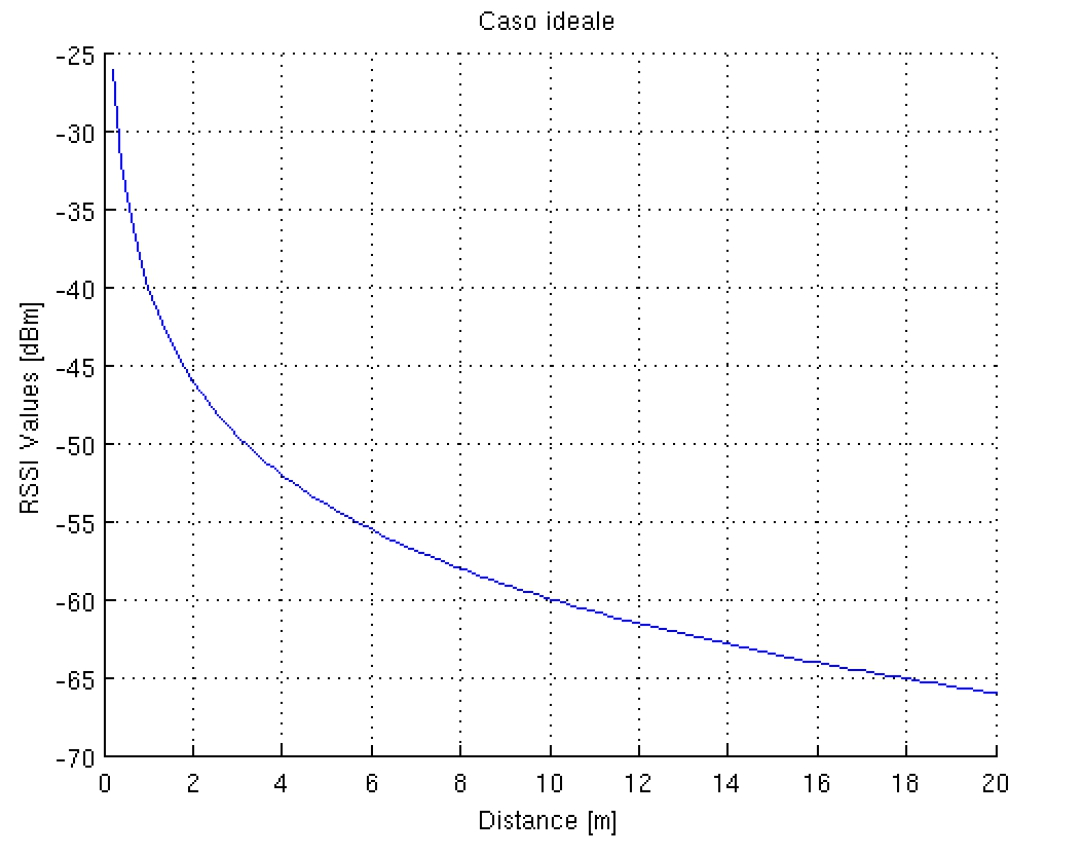
\includegraphics[scale=.25]{img/algoritmi/RSS.png}
	\caption{RSSI - Modello dell'andamento di RSSI in funzione della distanza}
\end{figure}



\section{Calcolo di RSSI}
Per il calcolo di RSSI (in dBm) si assume:
\begin{enumerate}
	\item che un segnale radio emesso in nello spazio libero da ostacoli e rumore decade di un fattore $ d^{-2} $, dove \textbf{d} è la distanza relativa trasmettitore-ricevitore
	
	\item che la potenza media ricevuta attraverso un canale reale decade proporzionalmente a $ n = d^{-n} $ , dove \textbf{n} è detto \textbf{l’esponente path-loss}. Tipicamente \textit{n} è compreso tra 2 e 4.
\end{enumerate}

\subsection{Equazione di trasmissione di Friis}

La distanza dal trasmettitore viene valutata utilizzando l’\textbf{equazione di trasmissione di Friis}:

\begin{equation}\label{eq:potenza_ricevuta}
P_R = P_T \frac{G_T G_R  \lambda^2}{(4 \pi)^2 \textbf{d}^n}
\end{equation}
dove:

\begin{itemize}
	\item $ P_R $ : potenza del segnale ricevuto (espressa in Watt) 
	\item $ P_T $ : potenza del segnale trasmesso (espressa in Watt) 
	\item $ G_R $ : guadagno dell’antenna ricevente
	\item $ G_T $ : guadagno dell’antenna trasmittente
	\item $\lambda = \frac{v}{f}$ : lunghezza d’onda
	\subitem $ v $ : velocità di propagazione
	\subitem $ f $ : frequenza dell'onda 
	\item $ d $ : distanza in metri
	\item $ n $ : constante di propagazione del segnale che dipende dall’ambiente
\end{itemize}
L'equazione \eqref{eq:potenza_ricevuta} calcola il rapporto tra la potenza ricevuta da un'antenna e la potenza trasmessa, in condizioni ideali.

\subsection{Conversione della potenza}
Conversione dalla potenza espressa in watt alla potenza espressa in dBm

\begin{equation}\label{eq:1dBm}
	1_{[dBm]} = 0.001258925_{[W]}
\end{equation}

\begin{equation}\label{eq:1W}
	1_{[W]} = 30_{[dBm]}
\end{equation}

\begin{equation}\label{eq:potenza_in_dBm}
	P_{[dBm]} = 10\log_{10} (10^{3}P_{[W]}/1_{[W]})
\end{equation}

\subsection{Potenza media a distanza di riferimento $ d_0 $}
\begin{equation}\label{eq:potenza_media_a_distanza_d}
	P(d)_{[dBm]} = P_{0\;[dBm]} \left(\frac{d}{d_0} \right)^{-n}
\end{equation}

dove $ P_0 $ è la potenza ricevuta (dBm) a una piccola distanza di riferimento $ d_0 $.

\subsection{Equazione di RSSI}
Combinando la \eqref{eq:potenza_ricevuta} e la \eqref{eq:potenza_in_dBm}, applicando le proprietà dei logaritmi si ottiene:
\begin{equation}
RSSI = −(10\,n\log_{10} \textbf{d} − A)
\end{equation}

dove \textit{A} è la potenza del segnale ricevuto (dBm) a distanza di un metro considerando una costante di propagazione \textit{n}.

\section{Calcolo della distanza}
La seguente equazione permette di stimare la distanza tra l'utente ed un target conoscendo il valore RSSI ed i parametri \textit{A} ed \textit{n}:

\begin{equation}\label{key}
RSSI = P - 10 * n * \log_10(d)
* n = 2 (in free space)
* d = 10 ^ ((TxPower - RSSI) / (10 * n))
\end{equation}

\begin{equation}
\textbf{d} = 10 \left( \frac{A − RSSI}{10\,n} \right)
\end{equation}

Con questa formula si può stimare la distanza .





\section{Problematiche della stima della distanza con RSSI}
I principali fenomeni negativi che inficiano l'utilizzo di RSSI come approccio per determinare la distanza tra due punti sono:
\begin{itemize}
	\item \textbf{Riflessione:} il segnale si propaga anche attraverso un percorso riflesso, provocando un \textbf{multi-path fading}. Al ricevitore giungono segnali con ampiezze e fasi differenti che vanno a sommarsi o sottrarsi in funzione della frequenza, causando un fading selettivo. Può essere causato da metalli e altri materiali riflettenti.
	\item \textbf{Intralcio:} shadowing che altera il normale decadimento dell’intensità che si avrebbe in spazio libero. L’attenuazione improvvisa del segnale è causata degli ostacoli (mobili, muri, alberi, edifici, ecc.) nel cammino trasmettitore-ricevitore
	\item \textbf{Assorbimento:} oggetti, come elementi liquidi o corpi umani, che assorbono la potenza del segnale.
	\item \textbf{Altezza:} la differenza di altezza può falsare la stima
	\item \textbf{Orientamento relativo:} il segnale decade se il ricevitore non è direzionato verso l'emettitore
\end{itemize}

\begin{figure}[!ht]
	\centering
	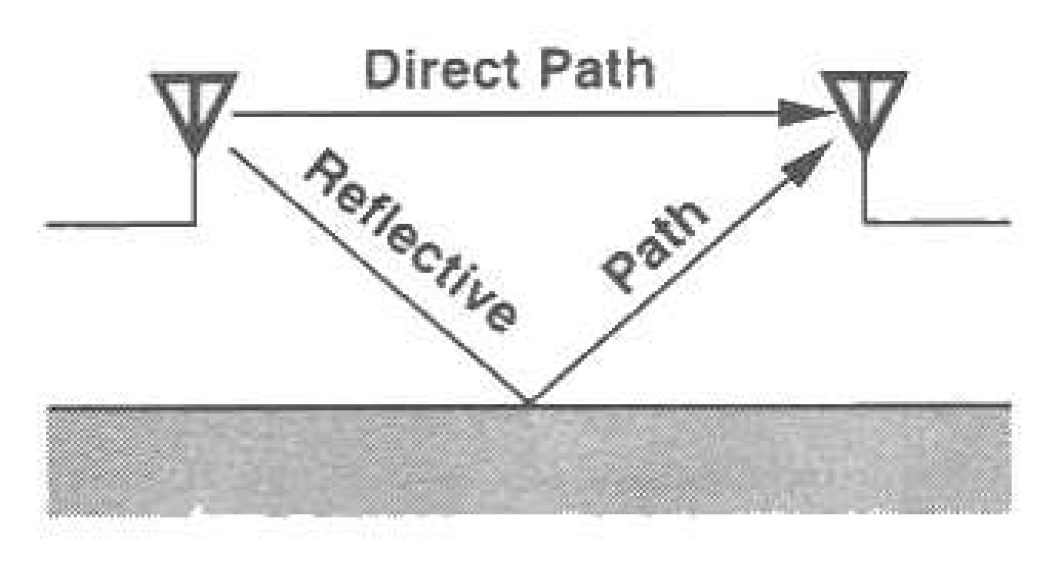
\includegraphics[scale=.16]{img/algoritmi/RSS_PROBLEMI.png}
	\caption{RSSI - Problemi di riflessione}
\end{figure}


 
 
